\chapter[Justificativa da abordagem]{Justificativa da abordagem}
  
    Com o passar do tempo, no mercado surgiram diversas abordagens para o desenvolvimento,
   as primeiras sendo chamadas tradicionais e, posteriormente, surgindo junto ao manifesto ágil,
   as adaptativas. Ambas abordagens possuem seus pontos fortes e fracos, dado esse fato veio a existir a necessidade
   de uma abordagem híbrida, de modo que quando necessário possam ser aproveitadas características de ambas as abordagens
   citadas, de acordo com \citeauthor{boehm} (\citeyear{boehm}).
  
  \section{Metodologia para a análise da abordagem a se utilizar}
   
   A complexidade intrínseca ao desenvolvimento de software e a variedade de métodos disponíveis dificultam
   a comparação entre as abordagens tradicionais e as adaptativas, tornando-a, muitas vezes, imprecisa \cite{boehm}.
   Todavia, Boehm e Turner (\citeyear{boehm}) levantaram algumas características dos projetos de software, as quais possuem diferenças
   visíveis entre os métodos ágeis e tradicionais. São elas:
  
   \begin{itemize}
    \item \textbf{Características da aplicação} – incluem objetivos primários do projeto, tamanho do projeto e o ambiente da aplicação;
    \item \textbf{Características do gerenciamento} – incluem relações com o cliente, comunicação no projeto e planejamento e controle;
    \item \textbf{Características técnicas} – incluem abordagens à definição de requisitos, desenvolvimento e teste;
    \item \textbf{Características das pessoas} – incluem características do cliente, dos desenvolvedores e da cultura da organização.
   \end{itemize}   
   
   As observações feitas por Boehm e Turner (\citeyear{boehm}) se consolidaram no levantamento de campos de domínio (\textit{home ground}) específicos
   para os métodos tradicionais e adaptativos, e na identificação de cinco fatores críticos que podem ser utilizados para 
   determinar como um projeto se relaciona com esses \textit{home grounds}.
      
    \pagebreak
    \subsection{\textit{Home grounds}}
      
      Os \textit{home grounds} (campos de domínio) de um método são os conjuntos de condições em que os métodos, tradicionais e
      adaptativos, tendem a se suceder melhor \cite{boehm}.
      
      \begin{citacao}
	O quanto mais longe as características de um projeto estiver do home ground de um método, mais arriscado é utilizar
	esse método puro como abordagem para o projeto e mais valioso é combinar esse método com algumas práticas complementares
	do método oposto. \cite{boehm}.
      \end{citacao}
      
      A tabela abaixo mostra as diferenças entre os métodos tradicionais e adaptativos,
      relacionando-as com as características de um projeto.
      
      \begin{figure}[!htbp]
	\centering
	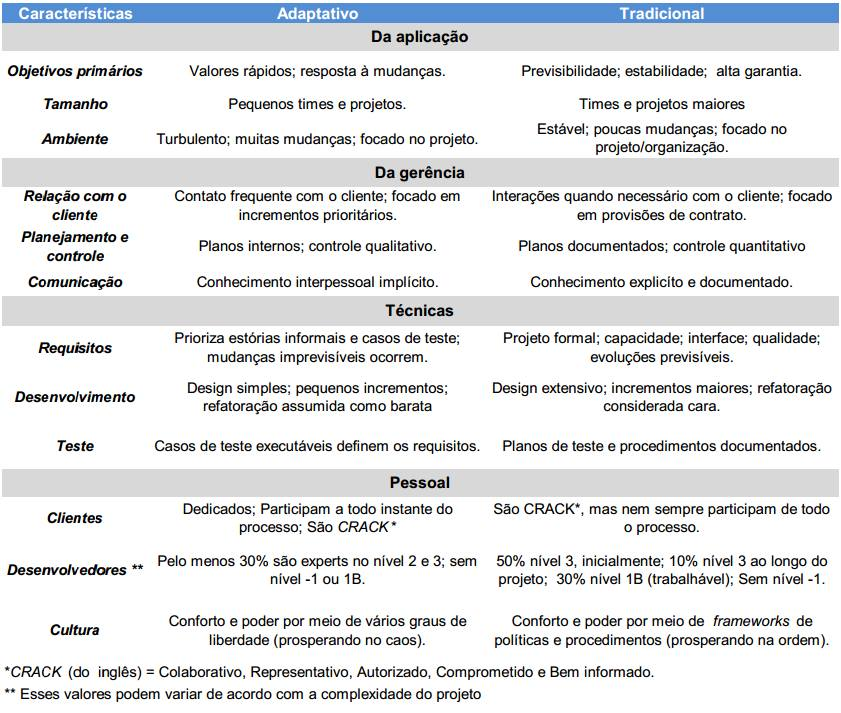
\includegraphics[scale=0.5]{editaveis/figuras/tabela_homegrounds_conceitos}
	\caption[Home ground ágeis e tradicionais]{Home ground ágeis e tradicionais.\footnotemark}
	\label{tabela_homegrounds_conceitos}
      \end{figure}
      \footnotetext{Fonte: \cite{boehm} }
   
    
    \pagebreak
    \subsection{Os cinco fatores críticos}
     
	\citeauthor{boehm} (\citeyear{boehm}) concluíram que existem cinco fatores críticos que determinam o encaixe de uma
	abordagem em determinado projeto. São eles: tamanho, criticidade, dinamismo, pessoal e cultura.
	
	O  fator tamanho diz respeito ao tamanho do projeto e do time. O fator criticidade diz respeito a quão crítico,
	intolerante à falhas, é o sistema. O fator dinamismo refere-se à mudanças inerentes aos processos de desenvolvimento
	de \textit{software}, diz respeito ao quão estável é o sistema.
	
	O fator pessoal refere-se às habilidades dos integrantes do time. \citeauthor{boehm} (\citeyear{boehm}) adaptaram
	o método da escala de classificação de habilidades de Cockburn para um método que caracteriza o pessoal necessário,
	em relação à capacidade de compreensão de um método de \textit{software} e a reação a determinado \textit{framework},
	em cinco níveis:
	
	\begin{itemize}
	 \item \textbf{Nível -1} - Nível de realocação. As pessoas devem ser rapidamente identificadas e realocadas para
	    trabalhar em algo que não esteja utilizando metodologias ágeis ou tradicionais. Podem ter habilidades técnicas,
	    porém não podem ou não estão dispostas a colaborar com o time ou seguir métodos compartilhados;
	 
	 \item \textbf{Nível 1B} - Nível em que a pessoa necessita de uma orientação considerável. As pessoas são medianas
	    e abaixo da média, com pouca experiência, todavia são desenvolvedores esforçados. Podem trabalhar bem no
	    desenvolvimento de software em uma situação estável, porém, é provável que atrasem um time ágil tentando
	    enfrentar uma mudança rápida (especialmente se forem a maioria do time). Trabalham bem em ambientes tradicionais;
	 
	 \item \textbf{Nível 1A} - Nível em que a pessoa necessita de orientação, porém trabalham bem em times ágeis.
	    As pessoas podem trabalhar bem tanto em times ágeis ou tradicionais, se houver pessoas suficientes do nível 2
	    para auxiliá-las. Com o tempo, podem vir a se tornar nível 2;
	 
	 \item \textbf{Nível 2} - Nível em que a pessoa pode gerenciar projetos pequenos ou em similares aos que já foram
	    feitos, porém precisam de pessoas do nível 3 para projetos grandes ou sem precedentes. Alguns possuem a habilidade
	    de se tornar nível 3 com o tempo, outros não;
	 
	 \item \textbf{Nível 3} - Capazes de revisar um método (quebrando sua regras) para se encaixar em uma situação
	    sem precedentes.
	\end{itemize}
	
      
	\begin{figure}[!htbp]
	  \centering
	  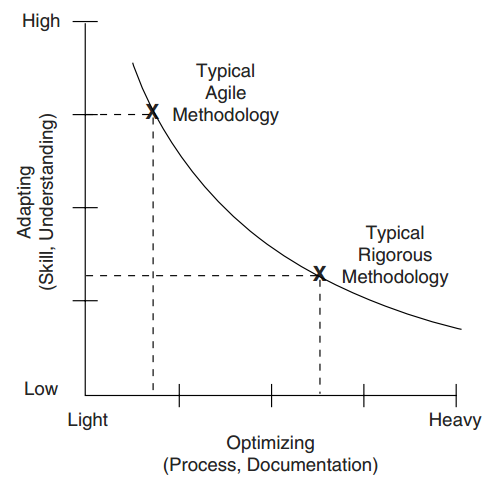
\includegraphics[scale=0.5]{editaveis/figuras/balancing_Optmizing_and_Adapting_Dimensions_graph}
	  \caption[Balanceando as dimensões de Otimização e Adaptação]
	    {Balanceando as dimensões de Otimização e Adaptação.\footnotemark}
	  \label{balancing_dimensions_graph}
	\end{figure}
	\footnotetext{Fonte: Cockburn e Highsmith (2000 \textit{apud} \citeauthor{boehm}, \citeyear{boehm}) }
	
	Ainda no quesito de pessoal, no que tange aos desenvolvedores, embora ambas abordagens, tradicional e adaptativa,
	trabalhem bem com uma variedade de desenvolvedores com diferentes níveis de habilidades e entendimento, a abordagem
	ágil tende a precisar de uma combinação mais rica de pessoas com níveis altos de habilidades (BOEHM e TURNER, 2004).
	A Figura~\ref{balancing_dimensions_graph} ilustra melhor esse preceito.
	
	O fator cultura refere-se ao “nível de liberdade” nos quais as pessoas envolvidas no projeto sentem-se confortáveis
	e seguras para definir e trabalhar problemas dentro da organização.

	Boehm e Turner (2004) forneceram um gráfico polar de cinco eixos que permite analisar visualmente a posição da
	abordagem adequada para um projeto, a partir da classificação do projeto ao longo dos cinco fatores críticos,
	avaliando os relacionamentos do \textit{home ground} do projeto.
	
	\begin{figure}[!htbp]
	  \centering
	  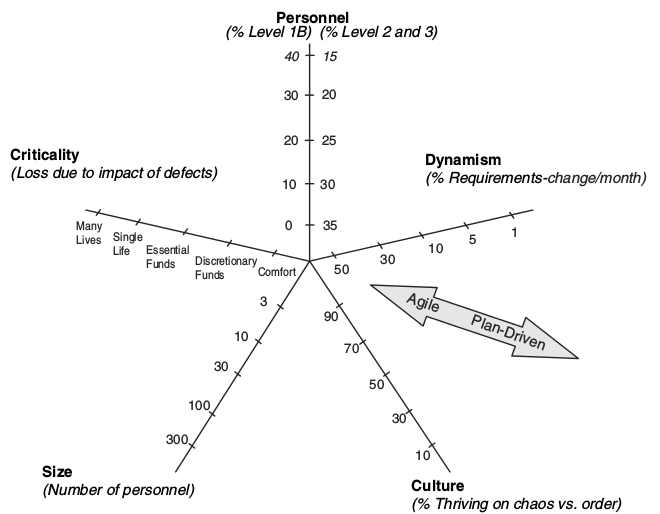
\includegraphics[scale=0.5]{editaveis/figuras/Dimensions_Afecting_Method_Selection}
	  \caption[Dimensões que afetam a seleção do método]{Dimensões que afetam a seleção do método.\footnotemark}
	  \label{five_dimensions}
	\end{figure}
	\footnotetext{Fonte: \cite{boehm} }
	
	Quanto mais ao centro as classificações, maiores serão as tendências adaptativas (ágeis), enquanto as tendências
	tradicionais se configuram mais aos extremos do gráfico. Se as classificações estiverem mais no \textit{home ground}
	de um método que do outro, ou bem divididas entre os métodos, seria necessário uma combinação entre os métodos para
	compor a abordagem adequada \cite{boehm}.
  
  \pagebreak
  \section{Proposta de abordagem}
    
    As características da equipe, da interação e do contexto de negócio foram analisadas sob a ótica dos pontos elucidados
    por Boehm e Turner (2004), já supracitados.
    
    A análise do contexto foi feita com o auxílio da Figura~\ref{homegrounds_nosso_projeto}. Comparou-se as características do projeto com os \textit{home grounds}
    dos métodos no intuito de mapear separadamente as características do nosso contexto nas possíveis abordagens.
    
    \begin{figure}[!htbp]
      \centering
      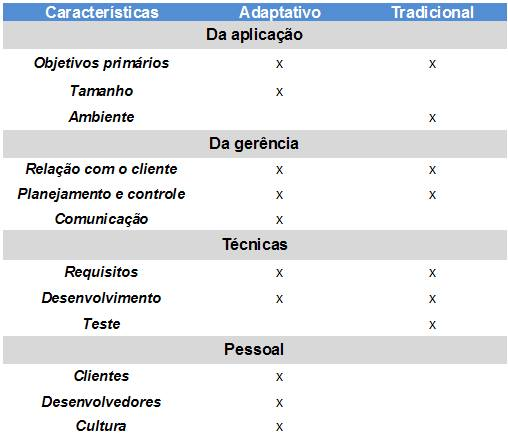
\includegraphics[scale=0.5]{editaveis/figuras/tabela_homegrounds_Nosso_contexto}
      \caption[Mapeamento das características do projeto com os home grounds dos métodos]
	{Mapeamento das características do projeto com os home grounds dos métodos.}
      \label{homegrounds_nosso_projeto}
    \end{figure}
    
    Com o mapeamento do contexto de negócio e equipe, fica um pouco mais explícito que ambos os métodos, tradicional
    e adaptativo, fornecem características importantes para definir a melhor abordagem para o projeto, já evidenciando
    que a utilização dos dois métodos se mostra plausível, pela dispersão das classificações entre os campos.
    
    Estimamos também as características do projeto no gráfico polar de cinco eixos proposto por \citeauthor{boehm} (\citeyear{boehm}),
    para uma análise visual dos resultados. A Figura~\ref{dimensions_nosso_projeto} mostra o gráfico preenchido com as
    características estimadas do projeto.
    
    \begin{figure}[!htbp]
      \centering
      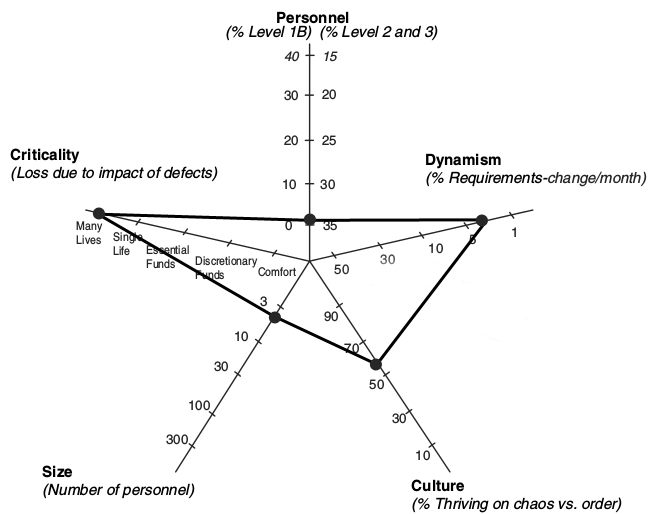
\includegraphics[scale=0.5]{editaveis/figuras/Dimensions_Afecting_Method_Selection_nosso_contexto}
      \caption[Análise das 5 dimensões para o contexto do projeto]{Análise das 5 dimensões para o contexto do projeto.}
      \label{dimensions_nosso_projeto}
    \end{figure}
    
    Analisando o gráfico, percebe-se que as classificações não se concentram majoritariamente nem nos extremos nem no centro
    do gráfico, evidenciando uma dispersão das classificações, com picos maiores em alguns eixos e picos menores em outros.
    Pelo que \citeauthor{boehm} (\citeyear{boehm}) colocaram, percebe-se a necessidade da combinação dos dois métodos, tradicional
    e adaptativo, formando uma abordagem híbrida.
    
    \subsection{Análise do contexto de negócio}
      
	O Corpo de Bombeiros Militar do Distrito Federal (CBMDF) é um órgão público que integra o Sistema de Segurança Pública,
	e é uma corporação bastante hierárquica estruturada em órgãos de direção, órgãos de apoio e órgãos de execução
	\cite{brasil91}.
	
	Como se trata de uma organização do setor público alguns aspectos são inerentes e se aplicam fortemente, como regimentos,
	leis e demais normas, necessidade de licitações para prestação de serviços, etc. Esses fatores, alinhado com a
	caracterização militar da organização, evidenciam a alta necessidade de formalização. Uma abordagem tradicional
	fornece melhores insumos para essa formalização \cite{boehm}.
	
	No quesito dinamismo, os métodos ágeis prosperam tanto com altas taxas quanto com baixas taxas de mudanças, enquanto
	os métodos tradicionais preferem baixas taxas de mudança para obterem êxito \cite{boehm}. Como na
	organização as taxas de mudanças são poucas, caracteriza-se um ambiente estável e pouco volátil, até pelo fato
	do regime militar e da carreira pública inerentes.
	
	Um fator que caracterizou bastante a classificação do território tradicional no gráfico, foi a criticidade do sistema.
	Como o sistema irá trabalhar com a gestão de viaturas, uma falha poderia acarretar, além de danos financeiros para a
	organização, complicações de saúde (ou até a morte) de uma pessoa que esperava por um atendimento de socorro,
	por exemplo, o que demonstra o quão crítico é o sistema, mesmo que indiretamente.
	
	
    \subsection{Análise da equipe}
	
	A questão da equipe foi um dos fatores que mais contribuíram para marcar o território ágil. Como a equipe é pequena
	(quatro integrantes), o modelo ágil do SAFe utiliza uma quantidade mínima de artefatos, papéis e práticas que são
	necessárias para a efetividade do time \cite{leffingwell11}. Embora os processos tradicionais possam ser adaptados
	para situações menores, essa adaptação não é algo fácil de se fazer, e geralmente é feita da maneira errada por uma
	pessoa que não é especialista no assunto, pois é necessário um nível de habilidade muito alto para tal
	\cite{boehm}.
	
	Como o projeto também não é de larga escala, a abordagem ágil permite uma dinâmica boa para a equipe.
	Embora a organização (CBMDF) seja demasiadamente hierárquica e complexa, a escalabilidade do SAFe permite suprir
	as necessidades que surgirem.
	
	A equipe chegou a conclusão que os integrantes estão classificados na escala de habilidades de Cockburn, adaptada
	por \citeauthor{boehm} (\citeyear{boehm}), entre os níveis 1A e 2, pois alguns integrantes possuem mais características para o
	nível 2 enquanto outros para o nível 1A, devido à experiências anteriores. Os métodos ágeis se adequam ao perfil
	do time, segundo os conceitos já apresentados por \citeauthor{boehm} (\citeyear{boehm}). Esse fator também justifica
	a classificação	no eixo da cultura, onde a cultura do time tende mais para o campo ágil.
	
	
    \subsection{Análise da interação com o cliente}
	
	Como a solução não irá servir apenas para o alto comando do CBMDF, várias patentes terão acesso restrito ao sistema,
	evidencia-se uma quantidade maior de \textit{stakeholders}. Para garantir a qualidade dos requisitos, um contato maior e
	constante com estes \textit{stakeholders} será um fator decisivo para a qualidade da solução. Esse ponto traz outra
	característica dos métodos ágeis para a proposta.
	
	Apesar da necessidade de ter um contato maior e constante com o cliente, o contexto da organização não permite
	o “abandono” de um contrato entre as partes. Por exemplo, para prestar serviços para o CBMDF é necessário uma
	licitação, onde estará descrita todas as cláusulas necessárias para o serviço que devem ser cumpridas. Nesse 
	ponto vemos que combinando a metodologia ágil com a tradicional, podemos responder melhor às mudanças e ainda
	assim cumprir provisões contratuais.
    
    \subsection{Considerações finais sobre a abordagem}
	
	Alguns órgãos públicos, ultimamente, estão querendo adotar os métodos ágeis em seu processo, mas também é impossível
	abrir mão das provisões contratuais e documentação exigidas em uma licitação, por exemplo.
	
	Como exemplo disto, basta analisar o edital de uma licitação feita pelo Corpo de Bombeiros do Estado de São Paulo
	no mês de abril de 2015, cujo objeto era a contratação de prestação de serviços de desenvolvimento e manutenção de
	software de sistemas de informação \cite{brasil15}.
	
	Foi colocado na licitação como critérios mínimos de avaliação da proposta técnica a utilização das
	“melhores práticas do mercado”, referindo-se as práticas da metodologia ágil, e ao mesmo tempo é solicitada
	uma documentação pesada com entregáveis obrigatórios, incluindo alguns conceitos típicos de abordagens tradicionais.
	
	Esse exemplo foi colocado apenas como ilustrativo da necessidade de uma abordagem híbrida, que era o que basicamente
	estava sendo pedido no edital da licitação como abordagem ágil. Lembrando que não significa que metodologias ágeis
	não façam uso da documentação ou de planejamentos, mas buscam documentar somente o necessário e fazer planos curtos,
	prefirindo explorar o conhecimento implícito das pessoas \cite{boehm}.
	
	Por fim, concluiu-se que a abordagem que melhor se adequaria ao contexto seria uma abordagem híbrida do
	\textit{Scaled Agile Framework} (SAFe), método ágil, com o \textit{Rational Unified Process} (RUP), método tradicional.